\documentclass[12pt]{article}
\usepackage[utf8]{inputenc}
\usepackage{amsmath}
\usepackage{mathtools}
\usepackage{amsfonts}
\usepackage{lastpage}
\usepackage{tikz}
\usepackage{pdfpages}
\usepackage{gauss}
\usepackage{fancyvrb}
\usepackage{fancyhdr}
\usepackage{graphicx}
\pagestyle{fancy}
\fancyfoot[C]{\footnotesize Page \thepage\ of 4}
\DeclareGraphicsExtensions{.pdf,.png,.jpg}
\title{MatIntroNat}
\author{Nikolaj Dybdahl Rathcke}
\chead{Nikolaj Dybdahl Rathcke (rfq695)}

\begin{document}
\section*{MatIntroNat - Ugeopgave 6}

\subsection*{Opgave 6.1}
Beregn
$$\frac{\mathrm{d}^2f}{\mathrm{d} y\mathrm{d} x}(x,y)$$
for funktionen $f(x,y)=y^2(1+xy)$. Beregn endvidere
$$\frac{\mathrm{d}^2f}{\mathrm{d}x\mathrm{d}y}(x,y)$$
Gør det samme for $g(x,y)=xy+cos(2x+y)$ og $h(x,y)=xln(x^2-2y)$. Tegner der sig et mønster?\\
En skal løses med Maple og en skal løses uden.\\
\\
For $f(x,y)$ starter vi med at differentiere for $x$ først.
$$\frac{\mathrm{d}f}{\mathrm{d} x}(x,y)=\frac{\mathrm{d}}{\mathrm{d} x}(y^2(1+xy))=\frac{\mathrm{d}}{\mathrm{d} x}(y^2+xy^3)$$
Vi kigger kun på leddene indholdende $x$, og derfor er
$$\frac{\mathrm{d}f}{\mathrm{d} x}(x,y)=y^3$$
Herefter differentieres resultatet efter $y$, og der fås at
$$\frac{\mathrm{d}^2f}{\mathrm{d} y\mathrm{d} x}(x,y)=3y^2$$
Herefter skal $\frac{\mathrm{d}^2f}{\mathrm{d}x\mathrm{d}y}(x,y)$ beregnes. Vi differentierer efter $y$ først
$$\frac{\mathrm{d}f}{\mathrm{d} y}(x,y)=\frac{\mathrm{d}}{\mathrm{d} y}(y^2+xy^3))=2y+3xy^2$$
Og resultatet differentieres for $x$, så vi finder det endelig resultat
$$\frac{\mathrm{d}^2}{\mathrm{d}x\mathrm{d}y}(y^2(1+xy))=\frac{\mathrm{d}^2}{\mathrm{d} x}(2y+3xy^2)=3y^2$$
\\
\\
Vi løser nu $\frac{\mathrm{d}^2g}{\mathrm{d} y\mathrm{d} x}(x,y)$ i Maple\\
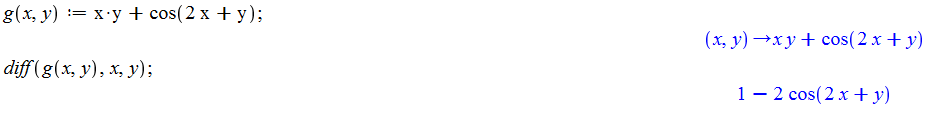
\includegraphics[scale=0.6]{Pic1}\\
og herefter $\frac{\mathrm{d}^2g}{\mathrm{d}x\mathrm{d}y}(x,y)$\\
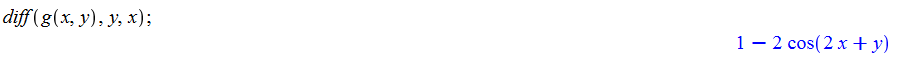
\includegraphics[scale=0.6]{Pic2}\\
Det samme gøres nu for $h(x,y)=xln(x^2-2y)$ med Maple, først $\frac{\mathrm{d}^2h}{\mathrm{d} y\mathrm{d} x}(x,y)$ \\
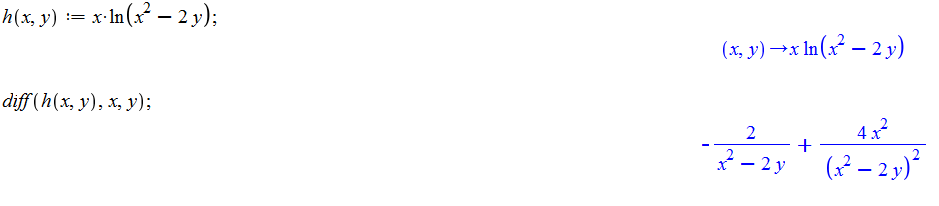
\includegraphics[scale=0.6]{Pic3}\\
Og herefter $\frac{\mathrm{d}^2h}{\mathrm{d} x\mathrm{d} y}(x,y)$\\
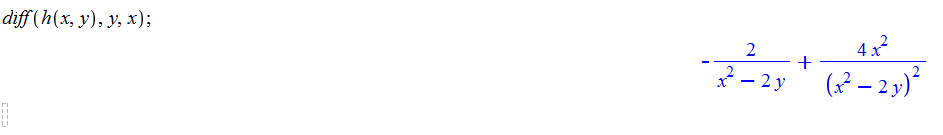
\includegraphics[scale=0.6]{Pic4}\\
Vi ser altså at rækkefølgen vi differentierer $x$ og $y$ i ikke betyder noget for de anvendte funktioner, da resultatet er det samme.

\newpage

\subsection*{Opgave 6.2}
Opgaven besvares uden Maple. Definer $h:\mathbb{R}^2\setminus\{(0,0)\}\rightarrow\mathbb{R}$ ved
$$h(x,y)=\frac{cosx-cosy}{x^2+y^2}$$
Bestem
$$H(x):=lim_{y\rightarrow0}h(x,y),\:x\in \mathbb{R},$$
for alle $x\in \mathbb{R}$. Er $H$ en kontinuert funktion af $x$?\\
Hvad siger dette om mulighederne for at vælge en værdi $c=h(0,0)$ sådan at $h$ bliver kontinuert i hele $\mathbb{R}^2$?\\
\\
Vi starter med at udregne $lim_{y\rightarrow0}h(x,y)$ for $x\neq0$.
$$lim_{y\rightarrow}h(x,y)=\frac{cosx-cos(0)}{x^2+0}=\frac{cosx-1}{x^2},\:x\neq0$$
Herefter beregnes $lim_{y\rightarrow0}h(0,y)$
$$lim_{y\rightarrow0}h(0,y)=lim_{y\rightarrow0}\frac{1-cosy}{y^2}$$
Dette giver et $\frac{0}{0}$ udtryk og vi benytter os derfor af L'Hôpitals regel
$$lim_{y\rightarrow0}h(0,y)=lim_{y\rightarrow0}\frac{1-cosy}{y^2}=lim_{y\rightarrow0}\frac{siny}{2y}$$
Da dette stadig er et $\frac{0}{0}$ udtryk bruger vi L'Hôpitals regel igen
$$lim_{y\rightarrow0}h(0,y)=lim_{y\rightarrow0}\frac{siny}{2y}=lim_{y\rightarrow0}\frac{cosy}{2}=\frac{cos(0)}{2}=\frac{1}{2}$$
Og vi har den endelige grænseværdi for $y\rightarrow0$ for $x\neq0$\\
Vi har nu funktionen
$$
H(x) = \left\{ \begin{array}{rl}
{\frac{cosx-1}{x^2}} &\mbox{ if $x\neq0$} \\
\frac{1}{2} &\mbox{ if $x=0$}
\end{array} \right.
$$
For at kunne sige at $H(x)$ er kontinuert for $x$ skal de have samme værdi i sammenfletningen, altså for $x=0$. Det vil sige at grænseværdien (fra begge sider) skal være lige $\frac{1}{2}$.
$$lim_{x\rightarrow0^-}H(x)=\frac{1}{2}\:\wedge\:lim_{x\rightarrow0^+}H(x)=\frac{1}{2}$$
Da $cos(x)$ nærmer sig $1$ for $x\rightarrow0$ lige meget hvilken side vi nærmer os fra, og at $x^2$ nærmer sig $0$ for $x\rightarrow0$ lige meget hvilken side vi nærmer os fra behøver vi ikke tage højde for hvilken side vi nærmer os fra det det giver samme resultat, altså skal vi blot finde
$$lim_{x\rightarrow0}\frac{cosx-1}{x^2}$$
Dette er et $\frac{0}{0}$ udtryk of vi benytter os derfor af L'Hôpitals regel.
$$lim_{x\rightarrow0}H(x)=lim_{x\rightarrow0}\frac{-sinx}{2x}$$
Dette er stadig et $\frac{0}{0}$ udtryk bruger vi L'Hôpital endnu en gang.
$$lim_{x\rightarrow0}H(x)=lim_{x\rightarrow0}\frac{-cosx}{2}=-\frac{1}{2}$$
Da dette $-\frac{1}{2}\neq\frac{1}{2}$ er $H(x)$ altså ikke en kontinuert funktion for $x$.\\
Dette vil sige at det ikke er muligt at vælge en værdi $c=h(0,0)$ så $h$ er kontinuert i hele $\mathbb{R}^2$, da afhængigt af hvilken vinkel vi nærmer os $h(0,0)$ fra kan vi få en vilkårlig $c$-værdi mellem $-\frac{1}{2}$ og $\frac{1}{2}$.

\end{document}
